\chapter{LFT: Computer Implementation}\label{ch:MCMC}

As discussed in \secref{sec:haar}, expectation values of 
physical observables $X$ in pure $\SU(N_c)$ LGT
are given by functional integrals
\begin{equation}\label{eq:exobs}
  \ev{X}=\frac{1}{Z}\int\DD{U}e^{-S(U)}X(U).
\end{equation}
Even though the integral~\eqref{eq:exobs} is well defined on a lattice
because there are 
finitely many sites, it is not feasible to evaluate it numerically; even
relatively small lattices have $4\times10^4$ links. The goal of our
simulation is to estimate $\ev{X}$ by randomly generating configurations,
distributed with probability $e^{-S}$,
and on each configuration, making a measurement $X_i$. The average 
\begin{equation}\label{eq:arithmeticaverage}
  \bar{X}=\frac{1}{\nconf}\sum_{i=1}^{\nconf} X_i
\end{equation}
serves as the estimator.

The strategy of carrying out a statistical computation using random sampling
goes under the name of {\it Monte Carlo}\index{Monte Carlo} 
algorithms\footnote{The idea of Monte Carlo algorithms dates back to the 1940s.
Stanislav Ulam wanted to know the probability of winning a game of Solitaire.
The calculation turned out to be too complicated to do by hand, so he wanted to
estimate this by playing repeated games, then calculating
$$
{\rm win\ chance}\approx\frac{\rm number\ of\ wins}{\rm number\ of\ games}.
$$
Of course this is tremendously tedious; it is much more appropriate for a
computer. Other scientists working with him at Los Alamos such as John von
Neumann and Nicholas Metropolis are early pioneers of this method.}.
The strategy of drawing these random configurations is to use a
Markov chain, and hence the backbone of a lattice calculation is
often referred to as {\it Markov chain Monte Carlo} (MCMC).
Further details on MCMC methods can be found in, for instance, 
Ref.~\cite{berg_markov_2004,gattringer_quantum_2010}. 


\section{Markov chain Monte Carlo}\label{sec:MCMCintro}

To generate our configurations, we start from some arbitrary configuration
$C_0$ and construct a stochastic sequence of configurations. 
Configuration $C_i$ is generated based on\index{update}
configuration $C_{i-1}$, which we call an {\it update} or {\it Markov
step}
The result is a {\it Markov chain}
\begin{equation}
  C_0\to C_1\to C_2\to...
\end{equation}
of configurations. 

\index{MCMC}
{\it Markov chain Monte Carlo} (MCMC) is characterized by the probability 
$W^{CC'}\equiv\pr{C'|C}$, the probability to jump to configuration 
$C'$ given that the system started in configuration $C$.
The MCMC {\it transition matrix}\index{transition matrix}
\begin{equation}
  W\equiv\Big(W^{CC'}\Big)
\end{equation}
is constructed to bring the system to {\it equilibrium}.
In equilibrium, the chain should have no sinks or sources of probability,
which means that the probability of jumping into a configuration $C'$
should be the same as jumping out of $C'$. This property
is called {\it balance}\index{balance}
\begin{equation}\label{eq:balance}
    \sum\limits_CW^{CC'}\pr{C}=
    \sum\limits_CW^{C'C}\pr{C'},
\end{equation}
with the LHS representing the total probability to end up in $C'$ and
the RHS representing the probability to transition out of $C'$.
If $W$ satisfies
\begin{enumerate}
  \item {\it ergodicity},\index{ergodic} i.e.
        \begin{equation}\label{eq:ergodicity}
          \pr{C}>0\;\;\text{and}\;\;\pr{C'}>0\;\;\Rightarrow\;\;
          \exists\;n\in\N\;\;\text{s.t.}\;\;\big(W^n\big)^{CC'}>0,
        \end{equation}
        which means that every possible configuration is accessible from
        any other configuration in a finite number\footnote{In practice,
        it's important that $n$ is not too large, otherwise some configurations
        will be sampled poorly. In a sense, this is the problem with
        topological freezing\index{topological!freezing}
        in \secref{sec:toplat}.} of Markov steps;
  \item {\it normalization},\index{normalization} i.e.
        \begin{equation}
          \sum\limits_{C'}W^{CC'}=1,
        \end{equation}
        which means that starting from configuration $C$ you have
        to move somewhere;
  \item and balance, 
\end{enumerate}
then the Markov process is guaranteed to bring the ensemble toward 
equilibrium. Using normalization, one finds from \equatref{eq:balance}
\begin{equation}\label{eq:eigenProb}
    \sum\limits_CW^{CC'}\pr{C}=\pr{C'},
\end{equation}
which shows that the equilibrium distribution is a fixed point of
the Markov chain\footnote{Above, we called $W^{CC'}$ a transition matrix.
Equation~\eqref{eq:eigenProb} shows that we can think of the equilibrium
distribution as an eigenvector of $W$ with eigenvalue 1. Each component
of this vector thus yields the probability of a particular configuration.}. 

\index{Metropolis step}
Here and the following two sections,
we omit the Lorentz index and space-time point from link variables to
avoid clutter.  We use $U$ to indicate the to-be-updated link, 
$U^\sqcup$ to indicate the staple matrix attached to $U$, and
$U'$ to indicate a trial link. We will use the Boltzmann
distribution $\pr{C}\propto e^{-S_C}$.

One trivial way to satisfy the balance condition~\eqref{eq:balance} is
to find an update that satisfies it term-by-term. For such an update, 
\begin{equation}\label{eq:detailedbalance}\index{detailed balance}
    W^{CC'}\pr{C}=W^{C'C}\pr{C'}.
\end{equation}
This property is known as {\it detailed balance}.
One of the most well-known Monte Carlo updates that satisfies detailed
balance is the {\it Metropolis algorithm}~\cite{metropolis_equation_1953}. 
In the Metropolis algorithm, a trial configuration $C'$ is selected 
with some probability distribution $\prt{C'|C}$. Then $C'$
is accepted with likelihood
\begin{equation}\label{eq:metupdate}
  \pr{C\to C'}=\min\left[1,\frac{\prt{C|C'}e^{-S_{C'}}}
    {\prt{C'|C}e^{-S_C}}\right],
\end{equation}
where $S_C$ is the action corresponding to $C$. 
If $C'$ is rejected, the unchanged configuration is counted
in the Markov chain. The total probability
to transition from $C$ to $C'$ using this strategy is 
\begin{equation}\label{eq:MCMCtransition}
W^{CC'}=\prt{C'|C}\pr{C\to C'}, 
\end{equation}
and using this fact, one
can show that this update satisfies detailed balance.

The Metropolis algorithm is in some sense the most standard Markov chain
algorithm used in lattice calculations, with the acceptance step
\equatref{eq:metupdate} being the most crucial part, in the sense that
it guarantees your configuration is drawn with the correct probability.
A Markov algorithm that concludes with the acceptance step is
said to be an\index{exact algorithm} {\it exact algorithm}\footnote{One
could imagine update steps that may not be guaranteed to draw configurations
from the desired distribution. This can be corrected by simply adding
the acceptance step at the end, and the algorithm is still exact.
One may neglect this acceptance step at the end, if one has reason to
believe the configuration is still drawn appropriately, but in such
instances the algorithm is not exact anymore.}.

In general, one could choose a trial configuration uniformly at random
from $\SU(N_c)$. On the other hand, as discussed above, if the trial
configuration increases the action substantially, then by
\equatref{eq:metupdate}, this trial is exponentially unlikely to
be accepted. If we are constantly suggesting such configurations,
we will make little movement in configuration space.
What makes an update efficient then is to suggest configurations that
have reasonable acceptance probabilities to begin with. This
strategy is often called {\it importance sampling}\index{importance sampling}.


\section{Update: Heat bath}\index{heat bath}

The {\it heat bath} (HB) algorithm takes this idea to the extreme. Here,
we construct our trial probability distribution to draw from the
Boltzmann distribution to begin with. Thus no formal accept/reject
step is required\footnote{The Kennedy-Pendleton algorithm has a sort
of accept/reject step on one of the random variables to ensure that
variable is drawn from the correct distribution.}. For pure gauge
simulations, it is common practice to generate a new configuration 
an old one by updating one link. 
For the $\SU(N_c)$ HB algorithm, the trial link distribution is
\begin{equation}\label{eq:PTdist}
  \dd{\prt{U'}}\propto \dd U'\exp\left(\frac{\beta}{N_c}\,\tr\,
  U'U^\sqcup\right).
\end{equation}
This construction also satisfies detailed balance. 
Numerically, the trick is to map \equatref{eq:PTdist} to a set
of real, random variables, which have to be specially
generated to reproduce the desired distribution.
A common strategy for doing this for the gauge group $\SU(2)$,
often referred to as the {\it Kennedy-Pendleton}\index{heat
bath!Kennedy-Pendleton} algorithm, is explained in an elementary way 
in Ref.~\cite{gattringer_quantum_2010}; the original papers are
Refs.~\cite{fabricius_heat_1984,kennedy_improved_1985}.

When $N_c>2$, this strategy is extended by leveraging the fact
that $\SU(2)\leq\SU(3)$; in general, an $\SU(N_c)$ matrix
can be broken down into $N_c(N_c-1)/2$ 
$\SU(2)$ submatrices~\cite{cabibbo_new_1982}. One generates each
$\SU(2)$ submatrix using the above HB, then reconstructs
the $\SU(N_c)$ matrix from those.

%Single link Metropolis or HB updates of links carried out in a systematic 
%(as opposed to random) order fulfill balance, but do not
%fulfill detailed balance.

\section{Update: Over-relaxation}\index{over-relaxation}

An additional useful update for $\SU(N_c)$ is the 
{\it over-relaxation}\index{over-relaxation} (OR) update. 
Adler introduced OR algorithms \cite{adler_over-relaxation_1981} and 
they were further developed by Creutz \cite{creutz_overrelaxation_1987} 
and others. The idea of the OR algorithm is to speed up relaxation 
by generating a group element ``far away" from $U$ without
destroying equilibrium, which is here achieved by keeping the action constant.
This update is not random in any way, but rather serves to move you around
in configuration space without impacting the acceptance rate too much.

More precisely let $U\in\SU(N_c)$ and suppose we have some method of
choosing another link variable $U_0$ that maximizes
the action for this staple.  We assume that this method of selection has no
dependence on $U$.  Pick some element $V\in\SU(N_c)$ such that $U=VU_0$; viewed
in this way, $U$ is ``on one side of $U_0$," and the element 
``on the other side" is $U'=V^{-1}U_0$.  Note that
\begin{equation}
  V=U U_0^{-1},
\end{equation}
which implies
\begin{equation}
  U' = U_0 U^{-1} U_0.
\end{equation}
This manner of constructing a new link variable $U'$, which generates
a group element ``far away" from $U$ without changing the action, 
is what we mean by over-relaxation.

In principle an OR update should be more efficient than a Monte
Carlo update. This is because we chose the new link variable to be two
group elements away from the old one, thrusting us further
along configuration space. However unlike Metropolis updates, OR updates 
only sample the subspace of constant action, and are therefore not ergodic. 
Hence to ensure an approach to equilibrium, they must be supplemented with, 
for instance, HB updates.

For $\SU(2)$, the update is given by
\begin{equation}\label{eq:ORupdate}
  U\to U'=\frac{1}{\det U^\sqcup}\left(U^\sqcup UU^\sqcup\right)^\dagger.
\end{equation}
\begin{proposition}{}{OR}\label{prp:OR}
  This update does not change the $\SU(2)$ Wilson action.
  \begin{proof}
   Since $\det(kA)=k^n\det A$ for any constant $k$ and $n\times n$ matrix $A$,
   one can show that the sum of two $\SU(2)$ matrices is proportional
   to an $\SU(2)$ matrix. Hence we can write
    $$
      U^\sqcup=u^\sqcup\sqrt{\det U^\sqcup}
    $$
    where $u^\sqcup\in\SU(2)$. After updating, the local contribution
    to the Wilson action becomes
    \begin{equation*}
      \tr U'U^\sqcup =\frac{1}{\det U^\sqcup}\tr
                       \left(U^\sqcup UU^\sqcup\right)^\dagger
                     =\tr U^\sqcup U\left(u^\sqcup\right)^\dagger u^\sqcup
                     =\tr U^\sqcup U,
    \end{equation*}
    which is what it was originally.
  \end{proof}
\end{proposition}
This simple 
behavior is special to $\U(1)$ and $\SU(2)$ LGT. 
For $N_c>2$, we again choose to do our efficient updates on
$\SU(2)$ submatrices of the original $\SU(N_c)$ matrix. 

\section{Update: Over-relaxation gauge fixing}\label{sec:ORgaugefix}

\index{gauge!fixing}
In general expectation values of gauge-dependent quantities are zero.
Nevertheless there are some rare occasions where it is useful to calculate
a quantity in a particular gauge, which can then be related to some
other physical quantity. In this section we cover an OR
algorithm that fixes gauge configurations to the {\it Coulomb} or 
{\it Landau} gauges.\index{gauge!Coulomb}\index{gauge!Landau}
In the continuum such gauges are given by the condition
\begin{equation}
  \partial_\mu A_\mu=0,
\end{equation}
where $\mu$ runs over only spatial directions for the Coulomb gauge, and
over all four directions for the Lorentz gauge. On the lattice, these 
{\it gauge conditions}\index{gauge!condition} are discretized as
\begin{equation}
  \Delta(x)\equiv A_\mu(x)-A_\mu(x-a\hat\mu) =0.
\end{equation}

\begin{proposition}{}{ORgf}
A gauge satisfying $\Delta(x)=0$ is achieved by extremizing
$$
  F\equiv-\Re\tr\sum_{x,\mu} g(x) U_\mu(x) g^\dagger(x+a\hat{\mu})
$$
\begin{proof}
Any gauge matrix can be written
$$
  g=e^{is^aT^a},
$$
where $s^a\in\R$ and $T^a$ are the generators of the Lie group. We want
to find the special $g_0$ that extremizes $F$; this is equivalent to finding
the $s_0$ that extremizes it. We will look in the vicinity of such a
gauge, i.e. look at gauges 
$$e^{i\tau^a T^a}, \qquad\tau\equiv s-s_0$$
with $\tau$ small. Then
\begin{equation*}\begin{aligned}
  F&=-\Re\tr\sum_{x,\mu}&&
      e^{i\tau^a(x)T^a}\,e^{iaA^b_\mu(x)T^b}\,e^{-i\tau^c(x+a\hat\mu)T^c}\\
   &\approx &&\big(\id+i\tau^a(x)T^a\big)
        \big(\id+iaA_\mu^b(x)T^b\big)
        \big(\id-i\tau^c(x+a\hat\mu)T^c\big)\\
   &\approx && \big(\id+a\tau^c(x+a\hat\mu)A_\mu^b(x)T^bT^c
                       -a\tau^a(x)A_\mu^b(x)T^aT^b\big),
\end{aligned}\end{equation*} 
where we have neglected $\order{a^2, a\tau, \tau^2}$ terms and use that
the $T^a$ are traceless. At the extremum, derivatives with respect to $\tau$
will vanish. Exchanging our dummy group summation indices and shifting
the first term by one site (which is allowed because of 
periodic BCs) we find
\begin{equation*}\begin{aligned}
  0=\pdv{F}{\tau^d}
     &=-\Re\tr\sum_{x,\mu}&&a\pdv{\tau^d}
        \left[A_\mu^b(x-a\hat\mu)\tau^c(x)-A_\mu^b(x)\tau^c(x)\right]T^bT^c\\
     &= &&a\left[A_\mu^b(x-a\hat\mu)-A_\mu^b(x)\right]T^bT^d.
\end{aligned}\end{equation*}
In order for the above to vanish, the term in brackets has to vanish,
which completes the proof.
\end{proof}
\end{proposition}
The strategy from here is to minimize $F$. As you can clearly see from
its definition, this can be accomplished through the replacement
\begin{equation}\label{eq:gfORupdate}
U\to U'=gU_\mu g^\dagger,
\end{equation}
which is reminiscent of the OR update~\eqref{eq:ORupdate}. Hence we employ
again OR, i.e. we find the $g$ minimizing $F$ and make the
replacement~\eqref{eq:gfORupdate}. In a similar strategy as
\propref{prp:OR}, we look at the local update to $F$,
\begin{equation}
  \Re\tr g(x)\sum_\mu\left[U_\mu(x)g^\dagger(x+a\hat\mu)
                        +U_\mu^\dagger(x-a\hat\mu)g^\dagger(x-a\hat\mu)\right]
  \equiv\Re\tr g(x)K(x).
\end{equation}
As before, $K(x)=\sqrt{\det K(x)}\hat K(x)$, where $\hat K(x)\in\SU(2)$.
To extremize $F$, we search for the $g$ rotating everything under the
trace to $\id$, which is clearly
\begin{equation}
  g(x)=K^\dagger(x)/\sqrt{\det K(x)}.
\end{equation} 

We will never achieve the condition $\Delta(x)=0$ on the computer exactly.
A measure of how close we are to satisfying the gauge condition is
\begin{equation}
  \theta\equiv\frac{1}{N_c N_s^3}\sum_x\tr\Delta(x)\Delta^\dagger(x).
\end{equation}
This combination is constructed so that $\theta\in\R$. 

For more information
about using OR to gauge fix, see Ref.~\cite{mandula_efficient_1990}. 
For information about how to implement this on multiple GPUs, see
e.g. Ref.~\cite{schrock_coulomb_2013}.

\section{Update: Molecular dynamics}\label{sec:MD}\index{molecular dynamics}

For this updating strategy, we leverage an isomorphism between
lattice field theory and a classical statistical mechanical 
ensemble. We will use this
correspondence to find a clever way of suggesting a gauge
configuration, and then ultimately accept or reject it via
a standard Metropolis step.

To start let's imagine a theory with a scalar field $\phi$ on 
the lattice. Then expectation values are computed like
\begin{equation}
\ev{X}=Z^{-1}\int\DD\phi e^{-S[\phi]}X[\phi],~~~~Z\equiv\int\DD\phi
e^{-S[\phi]}.
\end{equation}
Now let
\begin{equation}
H\equiv\frac{1}{2}\sum_{x\in\LAT}P(x)^2+S[\phi],
\end{equation}
where $P$ is a scalar field we will define in a moment. Since $P$ is some other
field, it follows that
\begin{equation}
\ev{X}=Z^{-1}\int\DD\phi\DD P e^{-H[\phi,P]}X[\phi],
~~~~Z\equiv\int\DD\phi\DD P e^{-H[\phi,P]}.
\end{equation}
Now let these fields evolve in Markov time $\tau$ and define
\begin{equation}
\dv{\phi(x)}{\tau}\equiv P(x).
\end{equation}
Then we have defined a classical system where $P$ is the momentum
conjugate to $\phi$. If we evolve $\phi$ and $P$ in $\tau$ according
to Hamilton's equations of motion, the energy is guaranteed to
be a constant. This procedure would yield 100\% acceptance if we
were able to integrate the equations of motion exactly. In practice
there is round off error, and the Metropolis step serves to protect
the probability distribution.

The above example is for a scalar field, which is a simplification of 
Ref.~\cite{callaway_microcanonical_1982},
which does it for $\U(1)$. This was shortly thereafter extended
to fermions~\cite{polonyi_microcanonical_1983}. 
This integration is completely deterministic, and hence does not
capture quantum fluctuations. To capture such quantum behavior,
one can intuitively imagine disturbing Hamilton's equations
with a random noise term. This is is an example of a
stochastic differential equation\footnote{A stochastic differential
equation is a differential equation where you include one
or more random forces. A simple example is the Langevin equation
$$
m \dv{v}{t}=-\lambda v+\eta(t)
$$
describing the Brownian motion of a particle of mass $m$
and velocity $v$ in a fluid. Here $\lambda$ is the drag, and
$\eta$ is a Gaussian-distributed noise term representing
random collisions of the particle with other particles in the fluid.
At a fixed value of the noise, such equations can be solved.
It becomes challenging when one wants to average over $\eta$.
}
like the Langevin equation, which can be used to model the inherent
randomness of the underlying quantum field 
theory~\cite{parisi_perturbation_1981}.
Inspired by this, we might consider to give the conjugate momentum
random kicks, following the microcanonical path in between.
This strategy is often called a 
{\it hybrid}~\cite{duane_hybrid_1985} strategy.
If not for numerical rounding error, this strategy would be expected
to generate the correct 
distribution~\cite{duane_theory_1986}.
To correct for numerical error, one can again apply the Metropolis
step as before, which is referred to as 
{\it hybrid Monte Carlo}\index{Monte Carlo!hybrid} (HMC).

Applying a series of molecular dynamics steps is usually called
a {\it trajectory}\index{trajectory}, after which comes the
Metropolis step. To fulfill detailed balance\footnote{Remember
we need this in order to ensure that the typical accept/reject
based on the configuration generated by the molecular dynamics
is a valid Metropolis step.}, we need to ensure
that our integration scheme
\begin{enumerate}
  \item preserves the integration measure $\DD\phi\DD P$; and
  \item is reversible.
\end{enumerate}
A commonly used scheme that fulfills these demands is known as the
{\it leapfrog} algorithm. Under this scheme, $\phi$ integrates
in $N$ steps of Monte Carlo length $\epsilon$, while $P$
starts with a step of length $\epsilon/2$, followed by $N-1$
steps of length $\epsilon$, and a final step of length $\epsilon/2$.
You can find an elementary proof that the leapfrog preserves area
and is reversible in Ref.~\cite{gattringer_quantum_2010}.
There one also finds a proof that the Metropolis fulfills detailed balance.

Let us synthesize what we have discussed to introduce an updating scheme that
represents a system of two indentical fermions with gauge interaction
at zero chemical potential.
This scheme for staggered fermions was first made explicit
in Ref.~\cite{gottlieb_hybrid-molecular-dynamics_1987}.
As discussed in \secref{sec:pseudofermions}, the most efficient way
to treat the determinant of the Dirac matrix is using pseudofermions.
Hence our path integral is\index{pseudofermion}
\begin{equation}\begin{aligned}\label{eq:twoFlavorRHMC}
Z&=\int\DD{U}\left(\det D\right)^2e^{-S_G}\\
&=
\int\DD{\Phi_R}\DD{\Phi_I}\DD{U} 
e^{-S_G-\Phi^\dagger\left(D^\dagger D\right)^{-1}\Phi},
\end{aligned}\end{equation}
where we have introduced a three-color, complex scalar field
$\Phi=\Phi_R+i\Phi_I$, the pseudofermion field.
In \secref{sec:pseudofermions} we stressed that the treatment of two identical
fermions was important since it lets us put a $D^\dagger D$ in the
exponential, which makes it a well defined probability distribution.
We also saw that we can draw our pseudofermions according to the
above distribution if we define $\Phi=D^\dagger R$ and draw $R$ from
$\exp\left(-R^\dagger R\right)$. The strategy then goes:
\begin{enumerate}
\item Generate Gaussian $R$.
\item Solve $\Phi=D^\dagger R$ to get $\Phi$.
\item Given your starting configuration $U$ generate conjugate
momenta.
\item Keeping $\Phi$ fixed, use the molecular dynamics strategy
to integrate along a short trajectory, yielding a proposal for $U$.
\item Do a Metropolis accept/reject at the end of the trajectory for $U$.
\end{enumerate}

Let us discuss steps 2-4 in a little more detail; in particular we would like to
understand how the molecular dynamics works for $\SU(3)$. We express our gauge
field as
\begin{equation}
U_\mu=e^{i\omega_\mu^aT^a}=e^{iA_\mu}.
\end{equation}
We will therefore think of our Hamiltonian as a function of the
generalized coordinates $A_\mu$, or equivalently when convenient,
$\omega_\mu^a$. The corresponding conjugate momenta are
\begin{equation}
P_\mu=P^a_\mu T^a.
\end{equation}
The steps taken in the leapfrog change the momentum. With our fictitous 
Hamiltonian in mind, what we seek is a force, i.e. a gradient of
the effective action. Looking at \equatref{eq:twoFlavorRHMC} our effective
action is
\begin{equation}
S_{\rm eff}=-S_G-\Phi^\dagger\left(D^\dagger D\right)^{-1}\Phi,
\end{equation}
and the force is
\begin{equation}
f=T^a\nabla^aS_{\rm eff}.
\end{equation}
The leapfrog thus proceeds in steps $\epsilon f$.

Based on the effective action, the force can be divided into the
{\it gauge force} and {\it fermion force}. The fermion force thus 
depends on the chosen discretization. For example with a straightforward Wilson
gauge action, whose contribution at $U$ has the form
\begin{equation}
-\frac{\beta}{6}\tr\left(UA+A^\dagger U^\dagger\right),
\end{equation}
where $A$ is the staple sum. Using \equatref{eq:lieDeriv},
the fact that the derivative lies in the Lie algebra,
which lets you express it as a linear combination of the generators,
and \eqref{eq:SUNnorm}, the gauge force comes out to be
\begin{equation}
f_G=-\frac{i\beta}{12}\left(UA-A^\dagger U^\dagger\right).
\end{equation}
Meanwhile, using \propref{prp:MATwrtSCLinv}, 
the fermion force can be written 
\begin{equation}
f_{\rm ferm}^a=
-T^a\left(\left(D^\dagger D\right)^{-1}\Phi\right)^\dagger
\left(\pdv{D}{\omega^a}D^\dagger+D\pdv{D^\dagger}{\omega^a}\right)
\left(\left(D^\dagger D\right)^{-1}\Phi\right).
\end{equation}
This shows that the inverse of $D^\dagger D$ must be computed
at each step of the molecular dynamics, which is far and away
the most expensive part.

Both here and in Step 2 we need to compute inverses of extremely
large matrices. One of the most efficient ways to approach this,
and indeed the strategy taken by codes such as 
QUDA, 
Grid, and
$\simulat$, is to use the conjugate gradient.
The difficulty of computing the inverse increases
substantially according to the smallest eigenvalue of $D$,
as mentioned in \secref{sec:numerics}. As a result
one may need to employ an SVD or a
{\it force filter}\index{force!filter}, which artificially
shifts low eigenmodes by an amount $\delta$.

\section{The HISQ force}\label{sec:HISQforce}

In this section we review aspects of computing the HISQ force specifically.
The HISQ action, discussed in \secref{sec:stagg} and \secref{sec:HISQ},
is widely used in state-of-the-art lattice calculations. Constructing its
force is a bit complicated, as it is a synthesis of many constructs in
those sections along with \secref{sec:MD}. 

We begin by writing down the action itself in a way that's helpful
for computer implementation. We write
\begin{equation}
S_f=\Phi^\dagger\left(D^\dagger D\right)^{-N_f/4}\Phi
=\bra{\Phi}\left(D^{\dagger} D\right)^{-N_f/4}\ket{\Phi},
\end{equation}
where $N_f$ is the number of fermions and $\ket\Phi$ is the pseudofermion field.
For this presentation of the HISQ force, we follow
Ref.~\cite{Wong:2007uz}, and hence switch to bra-ket notation.
Remember, we chose this pseudofermion rewrite to be able to compute the
determinant of the Dirac matrix efficiently. We want a
$D^\dagger D$ in the exponential since it has positive eigenvalues,
and hence makes for a well defined probability distribution.

The $D^\dagger D$ would correspond to two identical quarks of that flavor, since
by the Matthews-Salam formula
\begin{equation}
\det D^\dagger D = \det D^\dagger \det D
=\int \dd{\bar{\psi}_f}\dd{\psi_f}\dd{\bar{\psi}_g}\dd{\psi_g}
\exp\left(\bar{\psi}_fD^\dagger\psi_f+\bar{\psi}_gD \psi_g\right).
\end{equation}
The trick to get around this, as done in 
Ref.~\cite{gottlieb_hybrid-molecular-dynamics_1987}, is to define the
$\Phi$ fields on even sites only. This works because $D^\dagger D$ has no
matrix elements connecting even and odd sites. More precisely, if
$D_0$ is the massless part of the Dirac operator, then
\begin{equation}\begin{aligned}
\left(D^\dagger D\right)_{xy}
&=\left(2m\delta_{xz}+D^\dagger_{0,xz}\right)
  \left(2m\delta_{zy}+D_{0,zy}\right)\\
&=4m^2\delta_{xy}+2m\left(D^\dagger_{0,xy}+D_{0,xy}\right)+D^\dagger_{0,xz}D_{0,zy}.
\end{aligned}\end{equation}
The second term in the last line vanishes since $D$ is antihermitian.
The first term is diagonal in the site basis. Similarly $D$ itself always sends
odd to even or vice versa, so $D_0^\dagger D_0$ must preserve parity.
Hence if we write $D^\dagger D$ in a basis organized so even indices come first 
followed by odd, we have a block-diagonal matrix with two copies of
$4m^2+D_0^\dagger D_0$. Restricting to even or odd halves the number of degrees
of freedom, returning us once again to our interpretation of having a single
fermion species.

Finally we have the issue, discussed in
\secref{sec:HISQ}, that staggered fermions lead to four degenerate tastes.
The solution offered in that section is to take the fourth root. In practice,
this fourth root is implemented as a rational 
approximation~\cite{clark_rhmc_2004,clark_rational_2006},
\begin{equation}
\left(D^\dagger D\right)^{-N_f/4}\approx\alpha_0+\sum_l\frac{\alpha_l}{D^\dagger
D+\beta_l}.
\end{equation}
Using the rational approximation to estimate the fourth root in this hybrid
Monte Carlo scheme is called {\it rational hybrid Monte Carlo}\index{RHMC}
(RHMC).


Next we need to open up the $D$. We write\footnote{It is common practice in
lattice publications to use $M$ rather than $D$ to indicate the Dirac matrix.
In that case, $D$ is sometimes used to indicate the (covariant) derivative part.
I took the notation of Gattringer and Lang~\cite{gattringer_quantum_2010}.}
\begin{equation}\begin{aligned}
D(y|x)&=2m\delta_{x,y}
+\sum_\alpha \eta_\alpha(x)\left(\UHISQ_\alpha(x)\delta_{x,y-\hat\alpha}
-\left(\UHISQ_\alpha(x-\hat\alpha)\right)^\dagger\delta_{x,y+\hat\alpha}\right)\\
&\equiv 2m\delta_{x,y}+\dd_{x,y},
\end{aligned}\end{equation}
where $\UHISQ$ is given by \equatref{eq:HISQsmear}:
\begin{equation}
\UHISQ=\mathcal{F}^{\rm Fat7}_{\rm corr}\mathcal{U}\mathcal{F}^{\rm Fat7}U,
\end{equation} 
i.e. we Fat7-smear the thin link, followed
by a reunitarization and then a second-level smear that has some lattice-spacing
corrections built in. The $\eta_\alpha$ are the
staggered phases defined in \equatref{eq:staggeredPhase}.

\subsection{The Hasenbusch trick}\index{preconditioning!Hasenbusch}

At this point is has been mentioned multiple times that a major bottleneck
of the RHMC algorithm, which as of now is the fastest scheme for
generating configurations with dynamical quarks, is inverting the
Dirac matrix. As discussed in \secref{sec:numerics}, if this matrix
has a poor condition number, it is difficult to invert.
One way to alleviate this problem is to {\it
precondition}\index{preconditioning} the matrix. With this strategy,
we look out for a preconditioner $P$ to transform our to-be-solved equation to
\begin{equation}
DP^{-1}Px=b
\end{equation}
with the hope that $DP^{-1}$ has a better condition number than $D$ had.

Inverting $D$ becomes more costly as the bare quark mass is dialed down.
The {\it Hasenbusch trick}~\cite{hasenbusch_speeding_2001,urbach_hmc_2006}
notes that
\begin{equation}
\det D^{\dagger} D\left(m_l\right)=\det \frac{D^{\dagger}
D\left(m_l\right)}{D^{\dagger} D\left(m_h\right)} \det D^{\dagger}
D\left(m_h\right),
\end{equation}
where $m_l$ indicates some light quark mass and $m_h$ some heavier one.
The heavier masses are then treated with their own pseudofermion integrals.

\section{Choosing a random number generator}

As far as we know\footnote{See for instance \apref{ap:bell}.}, 
the only truly random or stochastic things in nature are
quantum mechanical measurements. This poses a problem for our strategy, since
we need a random number for the Metropolis step \equatref{eq:metupdate}.
In practice, one wants to generate a number $X$ uniformly at random
in the interval $X\in[0,1)$ and compute the number on the RHS
of \equatref{eq:metupdate}. If $X$ turns out to be greater, you reject $C'$.

In order to generate $X$, we use a {\it random number
generator}\index{generator!random number} or RNG. 
Since we cannot have a true random number\footnote{For
this reason, these algorithms are sometimes more aptly called
{\it pseudorandom number generators}\index{generator!pseudorandom number}
or PRNGs.}, we instead settle for an algorithm that produces a sequence of numbers
\begin{equation}
  X_{\rm seed},~X_1,~X_2,~...,~X_n,~...,
\end{equation}
by using some rule to generate $X_{n+1}$ given $X_n$. The starting number is
called the {\it seed}\index{seed}. The goal is to choose your rule so that,
given the seed, it is difficult or effectively impossible to figure out what
$X_n$ will be. Again, this is not a truly random process, but unfortunately it
is not yet practical to harness direct quantum-mechanical measurements to that
end. 

One of the earliest popular RNGs was the {\it linear congruence
generator}\index{generator!linear congruence}~\cite{lehmer_mathematical_1951,thomson_modified_1958}. 
Here the rule is pretty simple
to understand: You choose three tuning parameters $a$, $b$, $m\in\N$
and then generate according to
\begin{equation}\label{eq:linearCongruence}
X_{n+1}=(aX_n+b)\mod m.
\end{equation}
One can then convert a number $X_n$ generated in this way to a number $X$
in the unit interval as required for the Metropolis step by normalizing it by $m$.


\begin{figure}
\centering
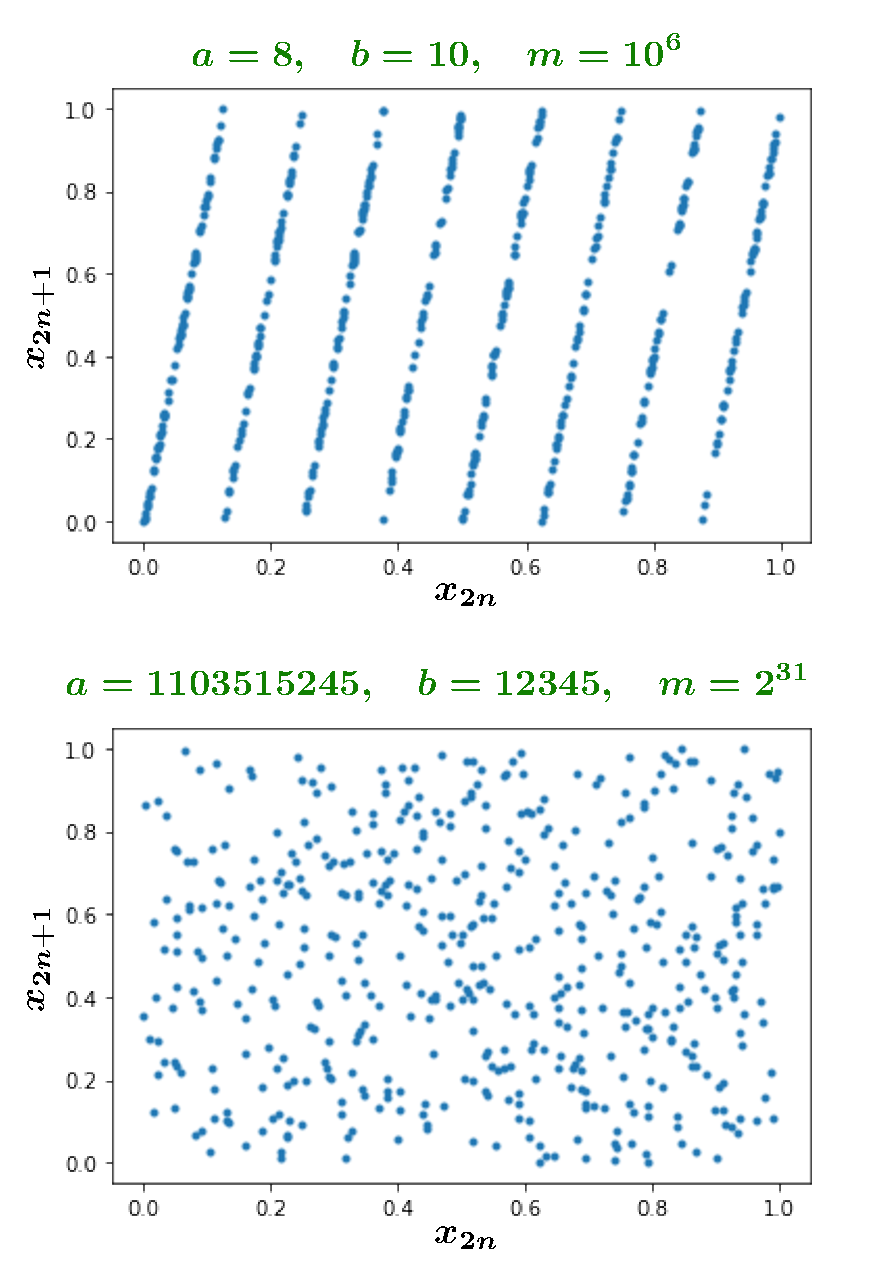
\includegraphics[width=0.6\linewidth]{figs/linear_congruence.pdf}
\caption{A strong correlation hidden in the linear congruence generator for
poorly chosen $a$, $b$, and $m$. Things seem to improve for a better choice of
these parameters, but as Marsaglia proved, this generator should be avoided. 
Image by C. Schmidt.}
\label{fig:LCG}
\end{figure}

The linear congruence generator is extremely easy to implement and is quite
fast. Unfortunately it suffers from one fatal flaw: It sucks. To see that it
sucks, one can plot $X_{2m}$ against $X_n$. An example of such a plot for
poorly chosen $a$, $b$, and $m$ is given in \figref{fig:LCG}. One sees the
pairs organize themselves into planes. Changing $a$, $b$, and $m$ seems
to improve the generator, but this flaw of the linear congruence generator
is fundamental. Indeed it was shown by Marsaglia~\cite{marsaglia_random_1968} that
outcomes of the linear will always arrange themselves in planes of hypercubes.
Hence one should never this generator for scientific purposes.

Looking for these hidden correlations is a bit challenging requiring some care
and experience. There are a variety of tests, but if you want to be thorough,
it is likely best to use already existing batteries, such as the {\it Diehard}
battery written by Marsaglia himself. More modern batteries, 
such as the {\it Dieharder}, can be found online~\cite{dieharder}.
Besides lacking hidden correlations, you would like numbers produced by your
RNG to match the target distribution. This can be quantitatively estimated
using, for instance, the Kolmogorov test of \secref{sec:kolm}.
Some modern RNGs that are known to be suitable for scientific purposes,
in particular passing some of the tests above, include
the\index{generator!Tausworthe} 
{\it hybrid Tausworthe}~\cite{tausworthe_random_1965,lecuyer_maximally_1996}
and\index{generator!Mersenne twister} 
the {\it Mersenne twister}~\cite{matsumoto_mersenne_1998}.

\section{Statistical analysis}\label{sec:statana}

Since $C_i$ is generated based on $C_{i-1}$, measurements on subsequent
configurations are correlated. In our simulations, these
correlations are reduced in two ways:
\begin{enumerate}
  \item Subsequent configurations are separated by multiple updating sweeps;
        and then
  \item configurations are grouped into $\nconf$ blocks or bins.
\end{enumerate}
The final measurements $X_i$ used in data analysis are obtained by averaging
within each block.
To check whether the final data are effectively independent, one can use
the integrated autocorrelation time. 
For statistically independent measurements, we expect the variance 
$\sigma^2_{\bar{X}}$ of $\bar{X}$ to be
\begin{equation}
  \sigma^2_{\bar{X}}=\frac{\sigma^2}{\nconf}
\end{equation}
due to the CLT. In practice, however, one finds 
\begin{equation}
  \sigma^2_{\bar{X}}=\frac{\sigma^2}{\nconf}\tauint.
\end{equation}\index{autocorrelation time!integrated}
The factor $\tauint$ is the integrated autocorrelation time. It is the 
ratio between the estimated variance of the sample
mean and what this variance would have been if the data were independent.
For effectively independent data, $\tauint=1$.

So, the final measurements are drawn from some
distribution with mean $\ev{X}$ and variance $\sigma^2$
and are effectively independent. The
estimator $\bar{X}$ of the mean is the average~\eqref{eq:arithmeticaverage}, 
while the unbiased estimator $\bar{\sigma}^2$ of the variance is
\begin{equation}\label{eq:estimatorvariance}
  \bar{\sigma}^2=\frac{1}{\nconf-1}\sum_{i=1}^{\nconf}
      \left(X_i-\bar{X}\right)^2.
\end{equation}
An estimator is biased if its mean for finite $\nconf$ 
does not agree with the exact result;
the bias is the difference. Generally, problems with bias emerge whenever
one wishes to estimate some non-linear function $f$ of the mean $\ev{X}$.
Naively one might guess
\begin{equation}
  \bar{f}_\text{bad}=\frac{1}{\nconf}\sum_{i=1}^{\nconf}f(X_i)
\end{equation}
as an estimator; however $\bar{f}_\text{bad}$ is not guaranteed
to converge to the exact result\footnote{See for instance the discussion
in \secref{sec:bias}.}. 
An estimator for $f(\ev{X})$ that converges to its true value is
\begin{equation}\label{eq:MCMCconsistentEst}
  \bar{f}=f(\bar{X});
\end{equation}
in particular, the bias of this estimator is $\order{1/\nconf}$.
Therefore in the large $\nconf$ limit, the bias vanishes faster than the 
statistical error bar.

At this point it is worth commenting when it is appropriate to use
the sample average~\eqref{eq:arithmeticaverage} and the estimator
\eqref{eq:MCMCconsistentEst}. The sample average is the preferred 
method to estimate an observable that can be directly calculated from 
the configurations, i.e. when $X_i=X(C_i)$. 
Such random variables are called {\it primary quantities},
\index{primary quantity} and they include many simple observables such
as the action, the absolute value of the Polyakov loop, and so on. 
However some quantities can only be calculated 
as functions of the sample average; these are called {\it secondary quantities}.
\index{secondary quantity} An obvious example is the variance, which is defined
only in terms of averages. But a less obvious example are particle masses,
which cannot be directly calculated on any single configuration. In this
case we are forced to use \equatref{eq:MCMCconsistentEst}.

We have introduced a way to estimate the mean and variance of some
operator, as well as a way to estimate the mean of some function of
that operator. Now we need a way to estimate the error bar of that
function. We cannot use
\begin{equation}
  \bar{\sigma}^2_{\bar{f}}=\frac{\bar{\sigma}^2_{\bar{f}}}{\nconf}
    =\frac{1}{\nconf\,(\nconf-1)}\sum_{i=1}^{\nconf}
     \left(f(X_i)-\bar{f}\right)^2
\end{equation}
because $f(X_i)$ is not a valid sample point.
One could analytically produce an error bar for $\bar{f}$ 
using error propagation. However when the function is complicated, 
error propagation becomes extremely unwieldy.

Jackknifing\index{jackknife} allows one to extract a mean and error bar,
and it is straightforward to implement; 
therefore it makes sense to use the jackknife method generally.
The idea of jackknifing is to throw away the first measurement, 
leaving $\nconf-1$ resampled values. Then we resample again, this
time throwing out the second point, and so on. The resulting
jackknife bins are
\begin{equation}
  X_{J,i}=\frac{1}{\nconf-1}\sum_{j\neq i}X_j.
\end{equation}
The jackknife estimator for $f(\ev{x})$ is then
\begin{equation}
  \bar{f}_J=\frac{1}{\nconf}\sum_{i=1}^{\nconf}f(X_{J,i}),
\end{equation}
while the estimator for the variance of $\bar{f}_J$ is
\begin{equation}
  \bar{\sigma}^2_{f_J}=\frac{\nconf-1}{\nconf}\sum_{i=1}^{\nconf}
    \left(f(X_{J,i})-\bar{f}_J\right)^2.
\end{equation}

In many instances, we will need to compare two estimates 
of the same quantity against each other and decide whether the difference 
between them is significant. This can happen, for example, if we want to
compare another group's results with our own. Let their result
be $\bar{X}$ with uncertainty $\sigma_{\bar{X}}$ and ours be
$\bar{Y}$ with uncertainty $\sigma_{\bar{Y}}$. Then the probability
that these two estimates differ by at least $D$ is
\begin{equation}\index{Gaussian difference test}
  q=\pr{|\bar{X}-\bar{Y}|>D}
    =1-\erf\left(\frac{D}{\sqrt{2
     \left(\sigma_{\bar{X}}^2+\sigma_{\bar{Y}}^2\right)}}\right)
\end{equation}
assuming $\bar{X}$ and $\bar{Y}$ are normally distributed with
the same mean. This is called a Gaussian difference test. 
The quantity $q$ is called the q-value.
In practice we take $q\leq0.05$ to be an indication of a possible 
discrepancy between $\bar{X}$ and $\bar{Y}$, keeping in mind that 
$q\leq0.05$ by chance one out of twenty times.

In practice, the true variances $\sigma_{\bar{X}}$ and $\sigma_{\bar{Y}}$
are not known. If one wishes to use the estimators $\bar{\sigma}_{\bar{X}}$
and $\bar{\sigma}_{\bar{Y}}$ instead, one can perform a {\it Student
difference test} or {\it t-test}\index{t-test} to investigate whether the 
discrepancy $D$ is due to chance. Suppose the estimate $\bar{X}$ comes from 
$M_{\text{conf}}$ data, while $\bar{Y}$ comes from $\nconf$ data.
Assume $\sigma_{\bar{X}}=\sigma_{\bar{Y}}$, which
happens when the sampling methods used are identical.
We introduce the random variable
\begin{equation}
  t=\frac{D}{\bar{\sigma}_D},
\end{equation}
where $D=\bar{X}-\bar{Y}$, and
\begin{equation}
  \bar{\sigma}^2_D=\left(\frac{1}{M_{\text{conf}}}+\frac{1}{\nconf}\right)
                   \frac{(M_{\text{conf}}-1)\,\bar{\sigma}_{\bar{X}}^2
                    +(\nconf-1)\,\bar{\sigma}_{\bar{Y}}^2}
                   {M_{\text{conf}}+\nconf-2}.
\end{equation}
Then the probability that these two estimates differ by at least $D$ is
\begin{equation}
 q=2
 \begin{cases}
 \,I\left(z,\frac{\nu}{2},\frac{1}{2}\right) & \text{for }t\leq 0, \\
 \,1-\frac{1}{2}\,I\left(z,\frac{\nu}{2},\frac{1}{2}\right) & \text{otherwise},
 \end{cases}
\end{equation}
where $I$ is the incomplete beta function, $\nu=M_{\text{conf}}+\nconf-2$,
and
\begin{equation}
  z=\frac{\nu}{\nu+t^2}.
\end{equation}

To estimate finite size corrections and carry out continuum limit
extrapolations, we need a way to fit data to curves.
Consider a sample of $\nsim$ Gaussian, independent data points $(X_i,Y_i)$,
where the $Y_i$ have standard deviations $\sigma_i$ and the $X_i$ have
no errors. For instance, if one is interested in a continuum limit
extrapolation, the $X_i$ are $\beta$ values while the $Y_i$ are
ratios of scales evaluated at that $\beta$.
We model these data with a fit that depends on some set
of $M$ parameters
\begin{equation}
  y=y(x;a),
\end{equation}
where $a=(a_1,...,a_M)$ is the vector of these parameters. Our goal
is to estimate the $a_j$.
Assuming that $y(x;a)$ is the exact law for the data, the probability
distribution for the measurements $Y_i$ is 
\begin{equation}
  f(y_1,...,y_{\nsim})=\prod_{i=1}^{\nsim}\frac{1}{\sqrt{2\pi}\sigma_i}
      \exp\left[\frac{-(y_i-y(x_i;a))^2}{2\sigma_i^2}\right].
\end{equation}
The probability that the data fall within a region near what was observed is
\begin{equation}
  \text{P}=\prod_{i=1}^{\nsim}\frac{1}{\sqrt{2\pi}\sigma_i}
      \exp\left[\frac{-(y_i-y(x_i;a))^2}{2\sigma_i^2}\right]dy_i.
\end{equation}
Our strategy for determining the correct fit will be to find the vector $a$
that maximizes the above probability. This happens when
\begin{equation}
  \chi^2(a)\equiv\sum_{i=1}^{\nsim}\frac{(y_i-y(x_i;a))^2}{2\sigma_i^2}
\end{equation}
is minimized. This strategy is an example of a {\it maximum likelihood method}.

We now describe an iterative method to search for the minimum of $\chi^2$.
Let $a_n$ be the vector of parameters for the $n\nth$ iteration.
As long as $a$ is in a small enough neighborhood of $a_n$, we can safely
approximate
\begin{equation}\label{eq:NRapprox}
  \chi^2(a)\approx\chi^2(a_n)+(a-a_n)\cdot b
           +\frac{1}{2}(a-a_n)\,A\,(a-a_n),
\end{equation}
where the coefficients of the vector $b$ and the $M\times M$ matrix $A$ 
are given by the first and second derivatives of $\chi^2$ evaluated at $a_n$.
In the {\it Newton-Raphson method}\index{Newton-Raphson}, the next 
iteration $a_{n+1}$ is
determined from the condition $\nabla\chi^2(a)|_{a=a_{n+1}}=0$,
which yields
\begin{equation}\label{eq:NR}
  a_{n+1}=a_n-A^{-1}b.
\end{equation}
If the approximation~\eqref{eq:NRapprox} is not good, one can instead move
a small step in the direction of the gradient by
\begin{equation}\label{eq:SD}
  a_{n+1}=a_n-c\,b,
\end{equation}
where $c$ is a constant that is small enough not to overshoot direction
of steepest descent. This is an example of a {\it steepest descent method}.
The Levenberg-Marquardt\index{Levenberg-Marquardt} 
method~\cite{levenberg_method_1944,marquardt_algorithm_1963} 
varies smoothly between~\equatref{eq:NR} and 
\eqref{eq:SD}. Steepest descent is used far from the minimum, and 
then it switches to the Newton-Raphson method when the minimum is approached.

\section{General code structure}

Now that we have introduced the general idea of MCMC, along with some specific
updating schemes, and complications for statistical analysis, we are ready 
to discuss the computer implementation. In this section we will discuss the
general code structure. In the following sections, we will address various
implementation details important for improving code performance and readability. 


As mentioned earlier, we design the simulation using {\it local updates}, which
means we update the links one at a time. This is done in a systematic order,
because there is some computational advantage compared to updating in a
random order~\cite{berg_markov_2004}. 
An updating {\it sweep}\index{sweep} updates every link on the lattice once. 
To maximize efficiency while maintaining ergodicity, it is common for pure
$\SU(2)$ algorithms to use
a combination of HB and OR updating. 


An MCMC simulation of LGT broadly consists of three essential steps:
\begin{enumerate}
  \item {\it Initialization}: The first thing to do is get everything ready for
        the simulation. This includes initializing the random number generator,
        and setting up an initial configuration.
  \item {\it Equilibration} or {\it thermalization}:
        \index{equilibration}\index{thermalization}
        To avoid over-sampling rare configurations,
        one must perform many sweeps to bring the system to its equilibrium 
        distribution. The structure of this section looks like 
        \begin{verbatim}
        do from n=1 to n=nequi 
          call MCMC update
        end do
        \end{verbatim}
  \item {\it Configuration generation}: One we are in the equilibrium
        distribution, we want to generate configurations on which we can
        perform measurements. To help reduce correlations between
        measurements, multiple updating sweeps are performed in between.
        This section is structured as
        \begin{verbatim}
        do from n=1 to n=nconf
          do from n=1 to n=ndiscarded
            call MCMC update
          end do
          save configuration 
        end do
        \end{verbatim}
  \item {\it Measurements}: Now that we have a good sample of configuration
        space, we are ready to perform measurements there. Some measurements
        can be take {\it in situ}, i.e. they are incredibly cheap and can be
        calculated the moment the configuration is saved. Measurements of this
        type include simple link products like the Polyakov loop. More expensive
        observables may require inverting a Dirac matrix thousands of times, 
        gauge fixing, or smoothing. For such observables it is better to
        have separate code that runs on the saved configurations. This
        code is structured as
        \begin{verbatim}
        do from n=1 to n=nconf
          take measurement 
        end do
        \end{verbatim}
\end{enumerate}



\bibliographystyle{unsrtnat}
\bibliography{bibliography}
